\documentclass[12pt,a4paper]{article}
\usepackage[utf8]{inputenc}
\usepackage[ngerman]{babel}
\usepackage{amsmath}
\usepackage{amsfonts}
\usepackage{amssymb}

\def \blattNr{06}

	%\usepackage{xcolor}%für die Farben

\usepackage{tikz}
\usetikzlibrary{arrows,automata}

\title{Formale Grundlagen der Informatik II - Blatt \blattNr}
\author{Vincent Dahmen 6689845  \and Mirco \and Tim Jammer 6527284}




\begin{document}

\maketitle{}

\section*{\blattNr .3}
\subsection*{1.}
\begin{align*}
B=\{
&\begin{pmatrix}
0\\0\\3\\0\\2
\end{pmatrix},
\begin{pmatrix}
0\\0\\3\\1\\1
\end{pmatrix},
\begin{pmatrix}
0\\0\\3\\2\\0
\end{pmatrix},\\
&\begin{pmatrix}
0\\5\\2\\0\\2
\end{pmatrix},
\begin{pmatrix}
0\\5\\2\\1\\1
\end{pmatrix},
\begin{pmatrix}
0\\5\\2\\2\\0
\end{pmatrix},\\
&\begin{pmatrix}
0\\10\\0\\0\\0
\end{pmatrix},
\begin{pmatrix}
8\\0\\0\\0\\0
\end{pmatrix},
\begin{pmatrix}
2\\7\\0\\0\\0
\end{pmatrix},
\begin{pmatrix}
6\\2\\0\\0\\0
\end{pmatrix}
\}
\end{align*}
Die Ersten Beiden Zeilen Beschreiben die Markierungern, bei denen c für unbeschränktheit in $p_4$ sorgt.\\
Die Letzte Zeile Beschreibt die möglichkeiten, bei denen der Zyklus a,b für unbeschränktheit z.b. in $p_3$ sorgt.

\subsection*{2.}
\subsubsection*{a)}
Für Alle Pfade Gilt, dass wenn es einen Fehler gab solange Fehler gilt, bis nicht Batterie Gilt. Und es gilt nicht für alle Pfade das irgentwann in der Zukunft Active gilt.
\subsubsection*{b)}
Für Alle Pfade gilt In jedem Punkt, das es einen Pfad gibt, auf dem irgentwann Active gilt.

\subsection*{3.}
Alle Etiketten sind $\in P(\{Locked,Battery,On,Error,Active\})$
\begin{align*}
E_S(c_0)&=\{Locked,Battery\}\\
E_S(c_1)&=\{Locked,Battery,On\}\\
E_S(c_2)&=\{Battery,On\}\\
E_S(c_3)&=\{Battery,On,Active\}\\
E_S(c_4)&=\{Locked,Battery,Error\}\\
E_S(c_5)&=\{Locked\}
\end{align*}
es ergibt sich (durch einfaches austauschen der Zustände durch ihre entsprechenden ettiketten):
\begin{align*}
 E_S(SS(M_{cell}))=&( \{Locked,Battery\}\{Locked,Battery,On\}\\
 &(\{Battery,On\}\{Locked,Battery,On\})^*\\
 &(\{Battery,On,Active\}\{Battery,On,Active\}^*\{Battery,On\})^*\\
 &(\{Locked,Battery\} + \\
 &(\{Battery,On,Active\}\{Battery,On,Active\}^*\\
 &\{Locked,Battery,Error\}\{Locked,Battery,Error\}^*\\
 &\{Locked\}\{Locked,Battery\})))^\omega
 \end{align*}

\subsection*{4.}
Ja, da $c_0\in Sat(f)$ gilt.

\subsection*{5.}
Nein, die Formel glt nicht.
Beispielsweise die rechnung
\[c_0c_1c_2c_3c_4c_5(c_0c_1c_2)^\omega\]
erfüllt die Formel nicht. in $c_4$ gilt Error, allerdings gilt danach nie wieder Active

\subsection*{5.}
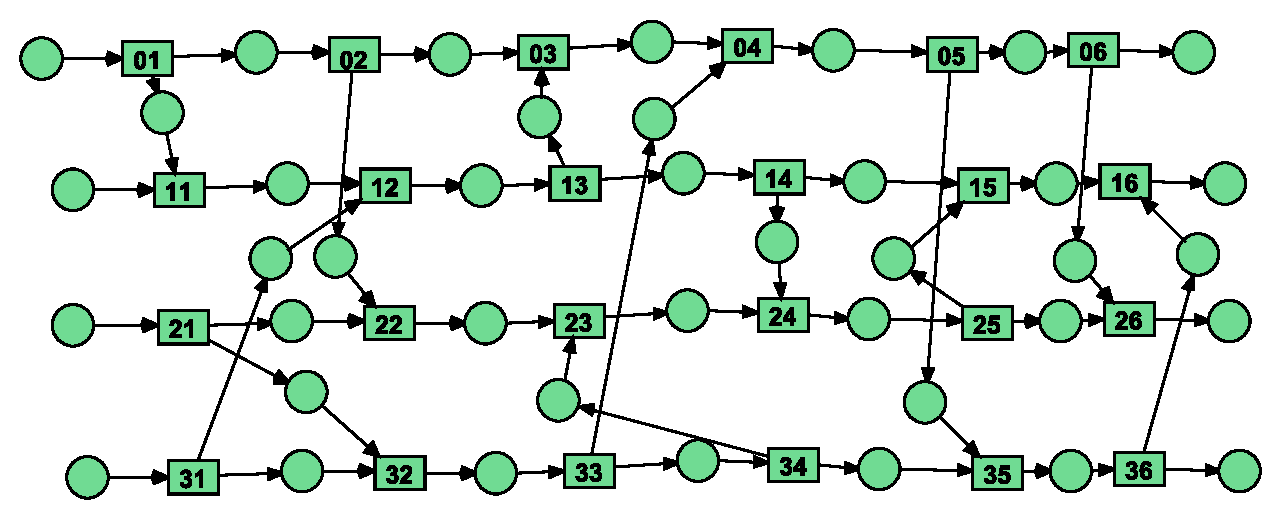
\includegraphics[scale=0.75]{Teilaufgaben/Aufgabe1-6.pdf}

\pagebreak

\section*{\blattNr .4}

\subsection*{1.}
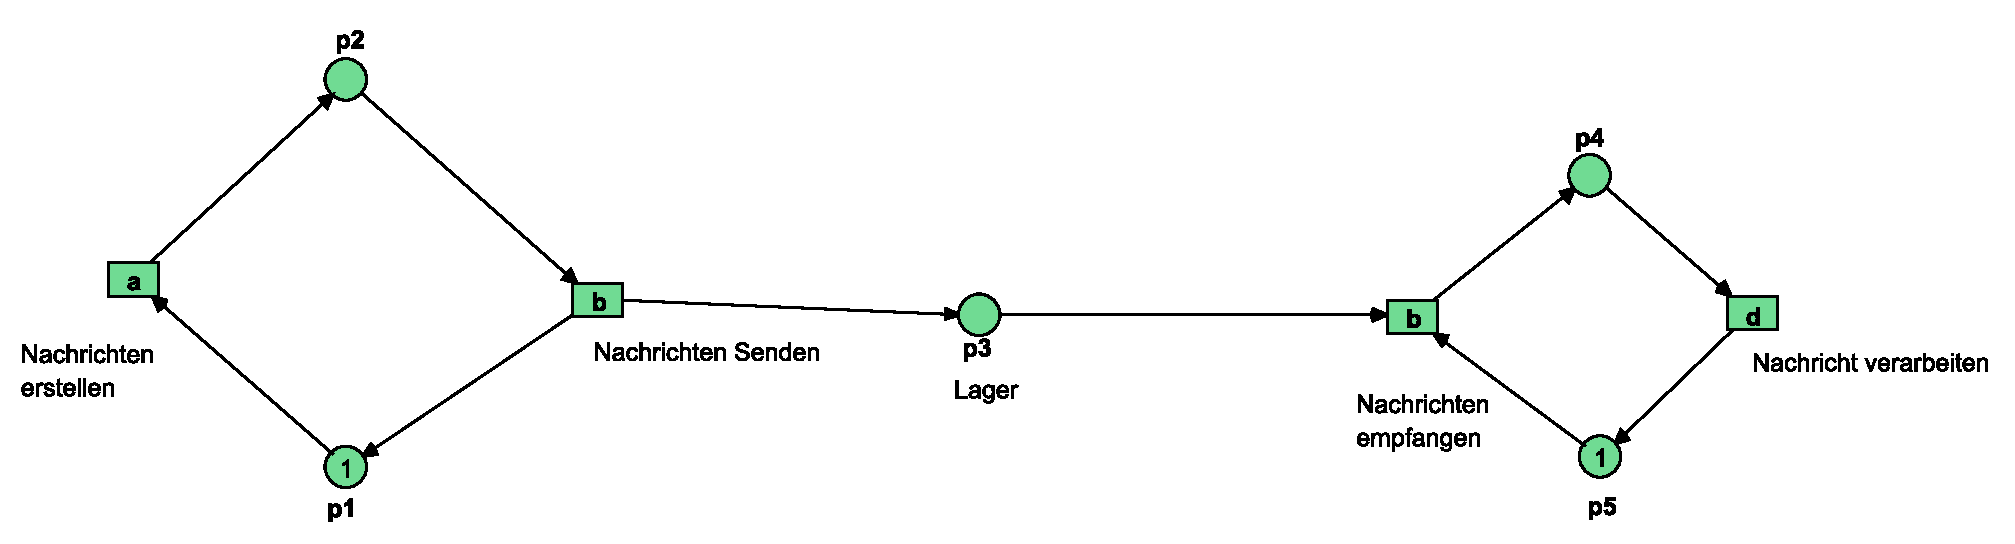
\includegraphics[scale=0.5]{Teilaufgaben/Aufgabe1.pdf}
%

%Alle Transtionssysteme sind Bisimilar:
\[TS_1 \underline{\leftrightarrow} TS_2: \mathcal{B}=\{(q_0,r_0),(q_1,r_1),...\}=\{(q_0,r_i)|i\  mod\  2 =0)\}\cup \{(q_1,r_i)|i\  mod\  2 \not = 0 \}\} \]

\[TS_1 \underline{\leftrightarrow} TS_3: \mathcal{B}=\{
(q_0,s_0),(q_1,s_1),(q_0,s_2),(q_1,s_3)\} \]

\[TS_2 \underline{\leftrightarrow} TS_3: \mathcal{B}=\{(r_0,s_0),(r_1,s_1)\}\cup \{(r_i,s_2)|i\  mod\  2 =0,\ i\geq 2)\}\cup \{(r_i,s_3)|i\  mod\  2 \not = 0,\ i\geq 3 \}\} \]

%
\subsection*{2.}
\includegraphics[scale=0.5]{Teilaufgaben/Aufgabe2.pdf}
%\begin{align*}
t_6&=(\underline{(b+b+b)}(\underline{(c+c)}+a) (c\underline{(d+d)}+\underline{(c+c)}\cdot \underline{(d+d)})\\
&=b(c+a) \underline{(cd+cd)}\\
&=b(c+a)cd\\
&=b(\underline{(c+a)cd)}\\
&=b(ccd +acd)\\
\end{align*}

$t_5$ und $t_6$ sind nicht äquivalent, da die normalformen unterschiedlich sind.


%
\subsection*{3.}
%\[(r+e+d)^*\cdot r\cdot e\cdot d\cdot(r+e+d)^*\]
auf die Klammern wurde, wo möglich, verzichtet
\includegraphics[scale=0.5]{Teilaufgaben/Aufgabe3.pdf}

\subsection*{4.}
%
\begin{tikzpicture}[->,>=stealth',shorten >=1pt,auto,node distance=2.8cm,
                    semithick]
  \tikzstyle{every state}=[fill=none,draw=black,text=black]

     \node[initial, state,accepting] (b1)[ below of=r1gr2]    {$B_1$};

  \node[state] (b2)   [ right of=b1]     {$B_2$}; 
     
  
   \node[state] (b3) [ right of=b2]	{$B_3$};  
     
 
    \node[state] (b4) [ right of=b3]	{$B_4$};
 
     
     
 
  \path   
  	  (b1) edge 	node {$rg_1,g_2$}	(b2)   	  
    
 	  (b2) edge 	node {$gr_1,r_2$} (b3)    
  	  
  	   	  (b3) edge 	node {$g_1,rg_2$}	(b4)    	  
  	  
  	  (b4) edge [bend left] node  {$r_1,gr_2$}	(b1)
  
  	
		;
        

\end{tikzpicture}
\includegraphics[scale=0.5]{Teilaufgaben/Aufgabe4.pdf}

\subsection*{5.}
\includegraphics[scale=0.5]{Teilaufgaben/Aufgabe5.pdf}
\\
oder\\
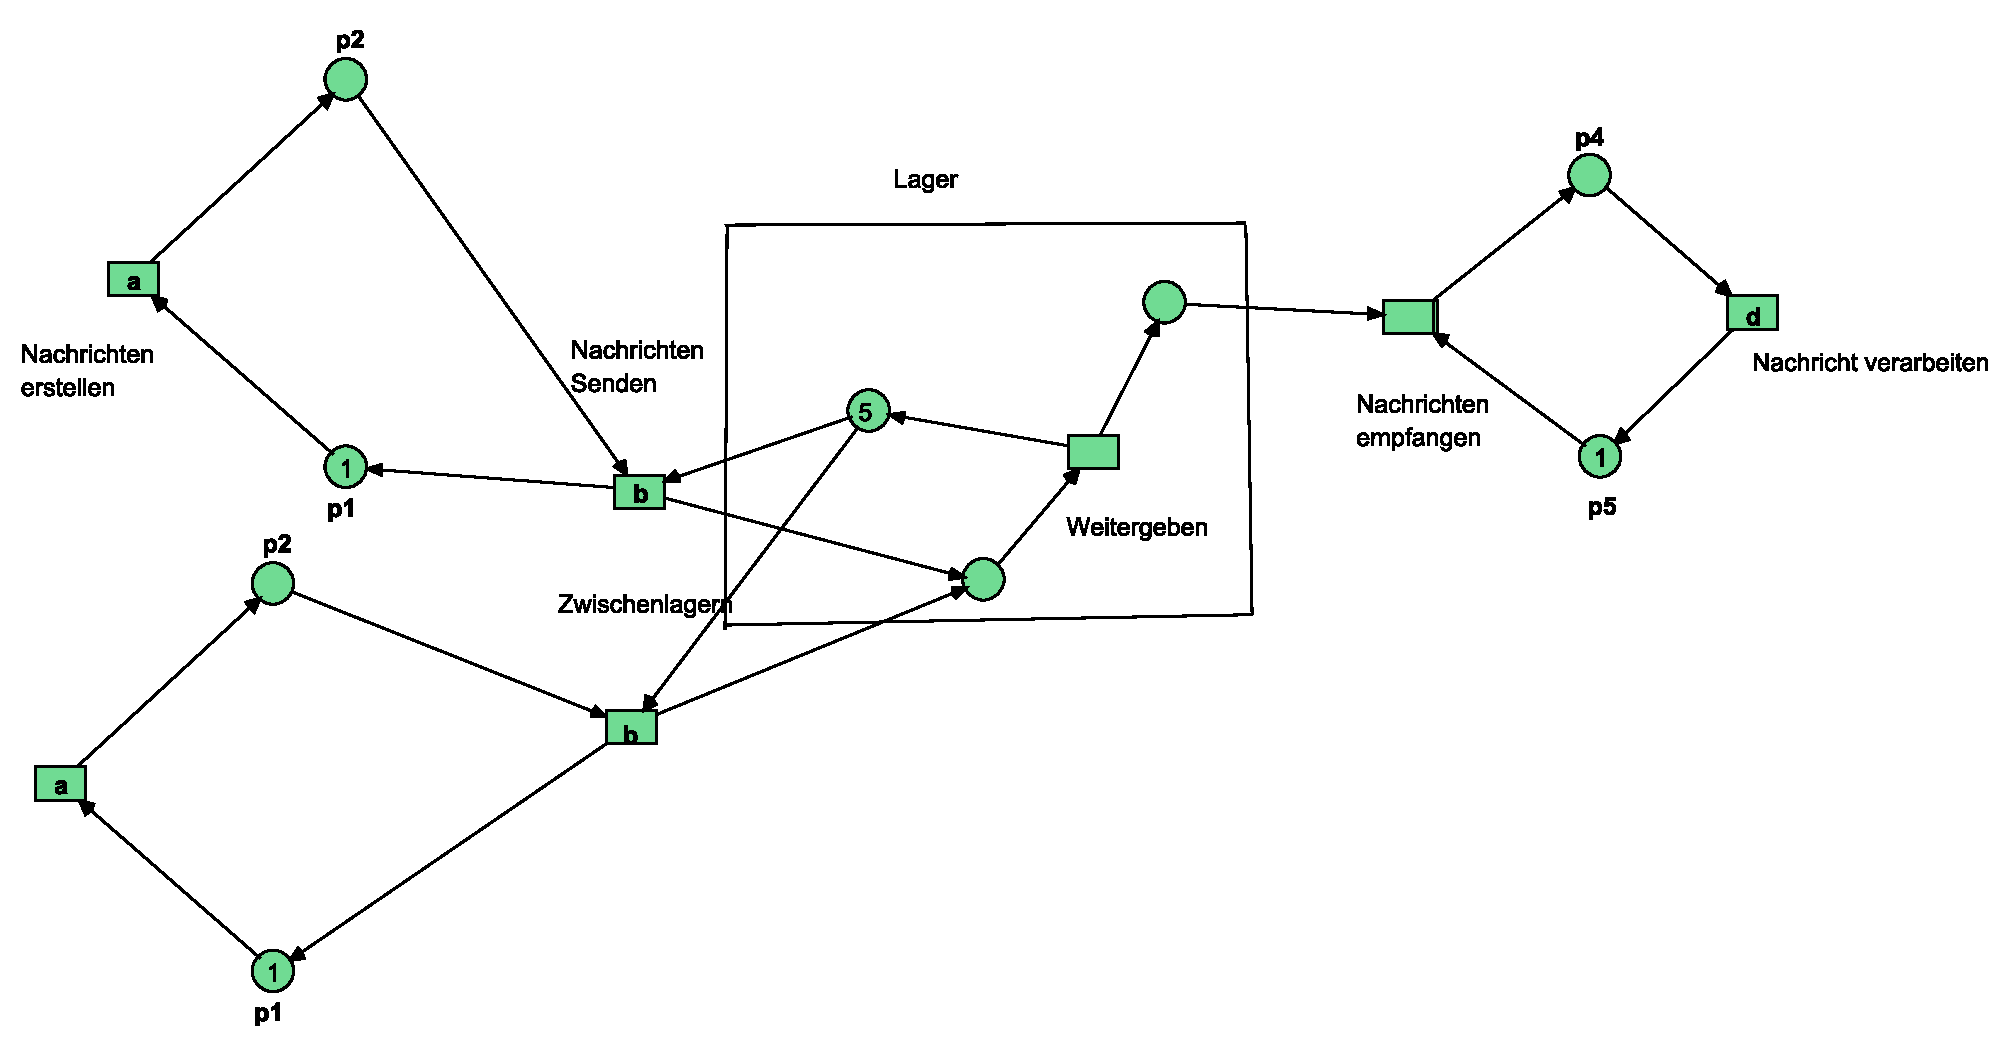
\includegraphics[scale=0.5]{Teilaufgaben/Aufgabe5Alternativ.pdf}
%
\begin{tikzpicture}[->,>=stealth',shorten >=1pt,auto,node distance=2.8cm,
                    semithick]
  \tikzstyle{every state}=[fill=none,draw=black,text=black]

     \node[initial, state] (b1m1)   {$B_1M_1$};

  \node[state] (b2m1)   [ right of=b1m1]     {$B_2M_1$}; 
     
  
   \node[state] (b3m1) [ right of=b2m1]	{$B_3M_1$};  
     
 
    \node[state] (b4m1) [ right of=b3m1]	{$B_4M_1$};
    
  \node[state,accepting] (b1m2)[ below of=b1m1]    {$B_1M_2$};

  \node[state] (b2m2)   [ right of=b1m2]     {$B_2M_2$}; 
     
  
   \node[state] (b3m2) [ right of=b2m2]	{$B_3M_2$};  
     
 
    \node[state] (b4m2) [ right of=b3m2]	{$B_4M_2$};
 
     
     
 
  \path   
  	  (b1m1) edge 	node {$rg_1,g_2$}	(b2m1)   	  
    
 	  (b2m1) edge 	node {$gr_1,r_2$} (b3m1)    
  	  
  	   	  (b3m1) edge 	node {$g_1,rg_2$}	(b4m1)    	  
  	  
  	  (b4m1) edge [bend left] node  {$r_1,gr_2$}	(b1m1)
  	  
  	  
  	  
  	    	  (b1m2) edge 	node {$rg_1,g_2$}	(b2m2)   	  
    
 	  (b2m2) edge 	node {$gr_1,r_2$} (b3m2)    
  	  
  	   	  (b3m2) edge 	node {$g_1,rg_2$}	(b4m2)    	  
  	  
  	  (b4m2) edge [bend left] node  {$r_1,gr_2$}	(b1m2)
  
  	
		;
        

\end{tikzpicture}
%
\subsection*{6.}
\includegraphics[scale=0.5]{Teilaufgaben/Aufgabe6.pdf}
%Da es Im Automaten keine Möglichkeit gibt, vom Start- zum Endzustand zu kommen, ist $L^\omega(B)\cap L^\omega(M)=\emptyset$ Damit ist die spezifikation erfüllt.

\end{document}
